\chapter{Design} \label{chapter:design}








\section{Návrh metód s MaFaulDa}
Súbor údajov MaFaulDa používame ako smerodajný pri určovaní metód schopných nasadenia na senzorovú jednotku. MaFaulda obsahuje 1951 záznamov so vzorkovaciu frekvenciu 50 kHz a označenými simulovanými poruchami rôznej závažnosti. Nahrávky obsahujú časové rady z dvoch trojosích piezoelektrických akcelerometrov. Po úprave ponechávame 6 typov značiek: referenčný bezporuchový stav, dve poruchy hriadeľa (nevyváženosť, nesúososť) a tri poruchy ložísk (poruchy klietky, guľôčok, vonkajšieho krúžku). 

Zo signálov rozdeleních na päť jednosekundových častí sa odstraňuje jednosmerná zložka odčítaním priemernej akcelerácie, po ktorej nasleduje dolnopriepustný 10 kHz filter. Z častí signálu je potom vytvorených 10 časových a 11 spektrálnych premenných. Euklidovská norma trojrozmerných atribútov eliminuje závislosť na smere merania. Pri výbere atribútov nie je do množiny pridaná taká dvojica, ak ich absolútna hodnota korelácie presahuje 0.95.

Predpokladáme, že dátové body rozprestreté v každej dimenzii priestoru môžu dobre rozlíšiť skupiny. Ukazuje sa, že premenné sú navzájom viac korelované v časovej doméne ako ilustruje analýza hlavných komponentov. Pre 95\% vysvetleného rozptylu PCA sú v časovej doméne potrebné 3 zložky, zatiaľ čo vo frekvenčnej doméne 4 zložky. PCA efektívne vyjadruje atribúty v menej rozmernom priestore, ale ich výslednou lineárnou kombináciou sa ťažko odôvodňujú rozhodnutia modelu.

Pri posudzovaní všeobecne najdôležitejších atribútov vychádzame z trojíc nekorelovaných atribútov vytvorených v 24 scenároch. Podmienky scenárov vznikli kombináciou štyroch kritérií: dávkové alebo inkrementálne učenie, pozícia ložiska, predikovaná premenná, limit na rotačnú rýchlosť. Na základe schvaľovacieho hlasovania sú najčastejšie sa vyskytujúcimi atribútmi v časovej doméne: špička-špička, faktor tvaru, faktor výkyvu. Vo frekvenčnej doméne sú to spektrálne ťažisko, roll-on a roll-off.

Tri typy experimentov s modelom k-NN prebiehajú s validáciou metódou hold-out, Najprv sa model naučí všetky extrahované prvky, takže nedochádza k výberu prvkov. Metódou hrubej sily sa hľadá kombinácia troch atribútov s najvyššou trénovaciou presnosťou. Následne sa porovnáva presnosť modelu pre tri atribúty zvolené technikami výberu atribútov. Dávkový model k-NN slúži ako referenčný, podľa ktorého sa posudzuje k-NN v postupnom učení.

Online učenie napodobňuje sťažené podmienky diagnostiky strojov, ktoré sa objavujú v praxi. Oneskorené dodanie alebo vynechanie skutočných značiek nepochybne znižuje spoľahlivosť klasifikácie. Modely k-NN v experimentoch s postupným učením sú trénované na rovnakom základnom súbore údajov pre ložisko A nad všetkými extrahovanými atribútmi. Týmto spôsobom môžeme porovnať trénovacie presnosti tréningu pre dávkové a postupné učenie. k-NN sme nastavili na 5 susedov a euklidovskú vzdialenosť. Metriky online učenia sa vyhodnocujú v metódou progresívnom vyhodnocovanie na ešte nevyváženom súbore údajov.

\section{Zber vibrácií v priemysle}
Doteraz uplatnená metodika pre súbor údajov zaznamenaných v laboratóriu sa aplikuje na vibračných signáloch z priemyselného prostredia. Pri monitorovaní zužitkujeme mierne prispôsobený postup z noriem. Ten zahŕňa výber strojov určených na monitorovanie, identifikáciu pozícií na meranie podľa technických štandardov, predbežné merania a vývoj senzorovej jednotky. Zber nového súboru údajov sprevádza vopred dohodnutý harmonogram.

Na zber údajov boli vyčlenené dva špirálové kompresory ako súčasť klimatizačných jednotiek pre dátové centrum a tri čerpadlá s troma elektrometrami v prečerpávacej stanici na pitnú vodu. Dlhodobejšie merania uskutočníme vlastným vnoreným systémom na báze vývojovej dosky ESP32-PoE-ISO so slotom na SD kartu. Ako senzor vibrácii použijeme MEMS akcelerometer IIS3DWB. Vyznačuje sa vysokou šírkou pásma až 6.3 kHz, nízkym šumom, a vysokou výstupným dátovým tokom 26.7 kHz cez SPI zbernicu.

\section{Záver}
V diplomovej práci sme sa zamerali na výber trendových ukazovateľov pre riešenie monitorovania prevádzkového stavu a odhaľovanie porúch z vibračných signálov.  Extrahované premenné pochádzajú hlavne z popisných štatistík, z článkov o spracovaní zvukových signálov a technických noriem vibrodiagnostiky.

Dosiahnuté stratové kompresné pomery pre MaFaulDa sú 2381:1 pre všetky atribúty a 25000:1 pre šesť atribútov. Výber atribútov metódou súčinu poradí zabezpečí väčšinou najlepšiu presnosť k-NN modelu oproti metrikám samostatne. Žiadny prístup však nedokázal nájsť trojicu prediktorov s presnosťou blízkou optimálnej, ktorá je až 98\%. Trénovanie k-NN na troch hlavných komponentoch prinieslo lepšiu presnosť ako výber atribútov. 

Model postupného učenia k-NN dosahuje prinajlepšom 90\% presnosť s okamžitou spätnou väzbou, 85\% so značkami oneskorenými o 250 pozorovaní a 82\% s iba 25\% anotovaného súboru údajov. Porovnateľný model trénovaný v dávkach dosahuje presnosť 98\%.  Doteraz boli urobené závery podľa súboru údajov MaFaulDa, ktoré plánujeme overiť na súbore údajov získaných v priemysle počas DP3.

% Features range (3D)
% Standing Fan
\begin{figure}[h]
    \centering
    \begin{subfigure}[b]{0.48\textwidth}
        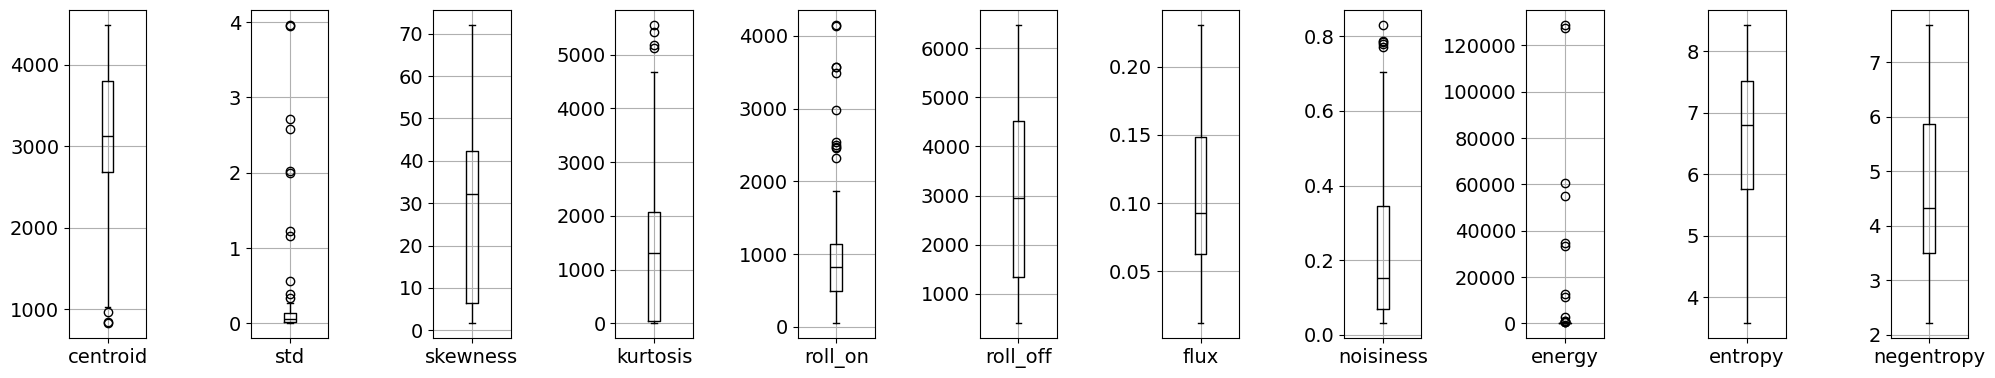
\includegraphics[width=\textwidth]{assets/results/feature-values/fan-TD-features.png}
        \caption{Time-domain features}
    \end{subfigure}
    \hfill
    \begin{subfigure}[b]{0.48\textwidth}
        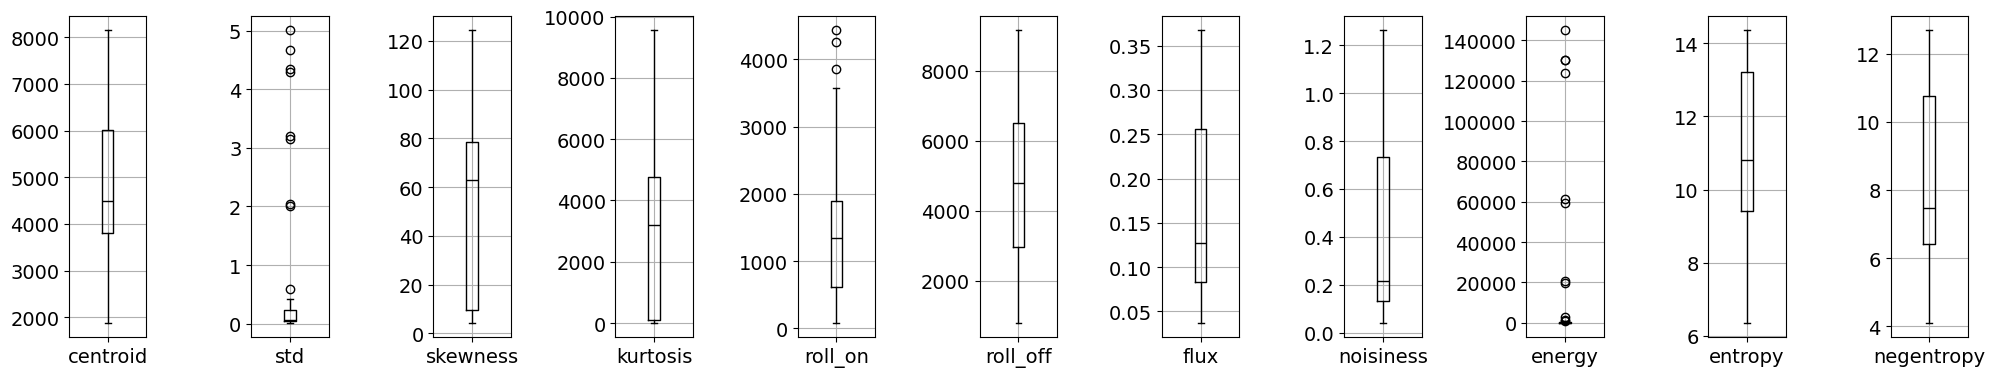
\includegraphics[width=\textwidth]{assets/results/feature-values/fan-FD-features.png}
        \caption{Frequency-domain features}
    \end{subfigure}
    \caption{Feature range in standing fan}
\end{figure}




%TODO ---------------------------------------------------------------------------
\section{Dataset exploration}
In establishing the viability of methods to be deployed on the sensor node, we explore the MaFaulDa dataset. It is the largest known machinery fault collection, so it is possible to create multiple subsets based on required conditions. 

One representative recording is first selected in each available fault category. The sample is visualized and statistically described in both temporal and spectral domains. A whole step-by-step procedure is outlined in the activity diagram (Fig.~\ref{fig:design:mafaulda-preprocessing}).

%\begin{figure}[ht]
%	\centering
%	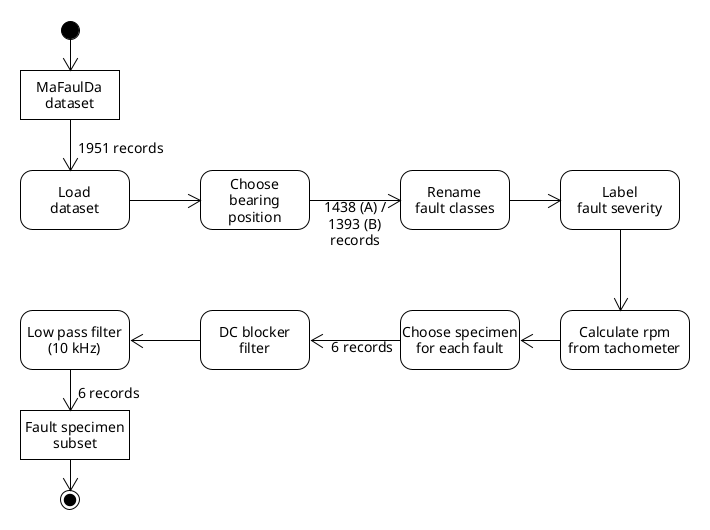
\includegraphics[width=\textwidth]{assets/design/activity-data-exploration.png}
%	\caption{Activity diagram of MaFaulDa dataset preprocessing}
%	\label{fig:design:mafaulda-preprocessing}
%\end{figure}

MaFaulda contains 1951 records labeled with inducted faults of increasing severity. The defects were set up on the machine simulator as is mentioned in the part about datasets. Time series of the triaxial piezoelectric accelerometers in separate files have a sampling frequency of 50 kHz. 

These vibration sensors are placed in two positions. The first placement is around the inner underhang bearing named \emph{A} which is closer to the motor. The second location is around the outer overhang bearing denoted as \emph{B} position.

\subsection{Feature selection}
The objective of feature selection is to find a subset of the most relevant predictors in each domain. As a starting point, the set consists of 3 non-correlated attributes under diverse conditions. Ultimately, a number of chosen features are to be tweaked to increase prediction accuracy. Four criteria are combined to put together 24 scenarios that filter rows from MaFaulDa:


In feature evaluation for fault prediction, we use hold-out validation in batch models and progressive valuation in online models. Classes in observations for batch models are rebalanced to the majority class with a random oversampling strategy. The training and testing set split ratio is 80 to 20. Classes for incremental learning are ordered by relative severity level and shuffled within levels. 

The best group of attributes is elected based on a training set with multiple methods. We compute the mean of the absolute value from point-biserial correlation, F statistic, and mutual information to the predicted variable. The features are then ordered in descending order by the received score. These individual ranks are combined by rank product to create an ensemble out of the metrics. Reference implementation of feature selection metrics uses Python packages Scikit Learn\footnote{SciKit Learn: \url{https://scikit-learn.org/}} in batch learning and RiverML\footnote{RiverML: \url{https://riverml.xyz/}} for online learning.


The choice of features is very sensitive to experimental conditions. Tendencies are demonstrated by counting how many triplets the indicator appears in across all possible situations. The results of approval voting are shown in Figure~\ref{fig:design:approval-rating-features}. The most occurring attributes in the temporal domain are zero-crossing rate, peak-to-peak distance, and average amplitude change. the features dominating in the spectral domain are centroid, roll-off, and roll-on.


\section{K-nearest neighbor classifier}
We utilize the k-nearest neighbor algorithm to check machinery diagnostics abilities with reduced feature sets. The k-NN classifier being a lazy learner means it can be adapted easily from offline to online context. Training labels are min-max scaled and establish nearest-neighbor decision boundaries for attribute values. Voronoi diagrams can display these regions and explain the model in that way. Batch learning in k-NN serves here as a target performance whose attainment is desirable with online learning.

\subsection{Batch models}
Three types of k-NN model experiments run with hold-out validation in a batch setting. First, the model learns all extracted features, so no feature selection occurs. Then, the brute-force method searches for a combination of three features with the highest training accuracy. In the end, the model performance for three attributes chosen by feature selection techniques is compared to principal components.


Two models are created for the target variable in classification with all 10 temporal and 11 spectral features. The subset of records includes all rotational speeds on bearing position A. Either six fault labels or anomalies above 0.9 severity level are guessed by the model with the same hold-out validation split as before. 

Confusion matrices for fault prediction and high severity anomaly are shown in Figure \ref{fig:design:KNN-confusion-matrix}. In this example, the number of k neighbors is 5, the distance metric is the Euclidian norm, and the algorithm for proximity queries is a k-d tree. The most inaccuracies in the temporal domain are between misalignment and bearing race faults. In the spectral domain, the model confuses imbalance and bearing faults because mass to unbalance is hung onto the shaft to cause bearing defects. 

In anomaly prediction, the error of the first degree is 7 times more prevalent than the error of the second degree. False positives are preferable, since we do not want the machine to fail prematurely and not know about it. In all cases, spectral features maintain better prediction metrics than all temporal features because of less interdependency among features. Bearing B exhibits overall worse classification performance because of more noise in the original signal.

Accuracies and F1 scores in both bearing positions with all extracted features are shown in Table \ref{tab:design:all-extracted-features}. Models are overtrained, especially for temporal features, because of the substantial difference between accuracy on training and validation sets. Binary classification of anomalies is unsurprisingly more precise in general than the multi-class case. Defect-type detection with all features reaches accuracy on the testing set above 98\% for bearing A, and above 90\% for bearing B.

Next, we exhaustively list all combinations of three features and look at the range of model performances generated. There are $\binom{n}{3}$ combinations of attribute triplets that entail 120 separate k-NN models for temporal domain features and 165 for the spectral domain. The feature set with the best evaluation scores serves as a benchmark for attributes picked by selection techniques. The accuracy of the k-NN algorithm for different target variables is in Figure \ref{fig:design:feature-combinations-KNN}. 



Features picked combinatorically for predictions are listed in Table \ref{tab:design:feature-combinations-KNN}. The worst accuracy occurs for temporal features in multi-class classification, 86\% and 77\% depending on bearing position, as compared to 98\% and 91\% accuracy for spectral features. An improvement would come with increasing the number of features, using a different base feature set with greater discriminatory power, or using a more sophisticated model.

\begin{table}[ht!]
\centering
\renewcommand{\arraystretch}{1.2}
\begin{adjustbox}{width=\textwidth}
\begin{tabular}{|r|r|r|l|r|r|}
\hline
\multicolumn{1}{|l|}{\textbf{Place}} & \multicolumn{1}{l|}{\textbf{\begin{tabular}[c]{@{}l@{}}Target \\ variable\end{tabular}}} & \multicolumn{1}{l|}{\textbf{Domain}} & \multicolumn{1}{l|}{\textbf{Best feature triplet}} & \textbf{\begin{tabular}[c]{@{}l@{}}Training \\ accuracy\end{tabular}} & \textbf{\begin{tabular}[c]{@{}l@{}}Testing \\ accuracy\end{tabular}} \\ \hline
\multirow{4}{*}{A} & \multirow{2}{*}{\begin{tabular}[c]{@{}r@{}}anomaly\\ (0.9)\end{tabular}}              & temporal        & \{zero-crossing, aac, rms\}         & 0.9843                & 0.9792 \\ \cline{3-6} 
                   &                                               & spectral        & \{centroid, noisiness, entropy\} & 0.9818                & 0.9707               \\ \cline{2-6} 
                   & \multirow{2}{*}{fault}                        & temporal        & \{zero-crossing, aac, rms\}         & 0.9701  & 0.9475 \\ \cline{3-6} 
                   &                                               & spectral        & \{centroid, kurtosis, entropy\}  & 0.9750                & 0.9505               \\ \hline
\multirow{4}{*}{B} & \multirow{2}{*}{\begin{tabular}[c]{@{}r@{}}anomaly\\ (0.9)\end{tabular}}               & temporal        & \{zero-crossing, aac, rms\}            & 0.9570                & 0.9227 \\ \cline{3-6} 
                   &                                               & spectral        & \{centroid, std, roll-on\}      & 0.9495                & 0.9185               \\ \cline{2-6} 
                   & \multirow{2}{*}{fault}                        & temporal        & \{zero-crossing, aac, rms\}     & 0.9173 & 0.8738 \\ \cline{3-6} 
                   &                                               & spectral        & \{centroid, std, roll-off\}     & 0.9067                & 0.8584               \\ \hline
\end{tabular}
\end{adjustbox}
\caption{Features with the highest accuracies on the training set found combinatorically}
\label{tab:design:feature-combinations-KNN}
\end{table}

The features picked using the rank product method are shown in Table \ref{tab:design:best-3-features-KNN}. Their prediction accuracies in k-NN models are subpar to optimal sets. However, the advantage is that the feature election process is not so computationally taxing. On bearing A, validation set accuracies for fault diagnostics are 85\% and 92\%, for each of the domains. Because of the low k hyperparameter value, models are overtrained either way.

\begin{table}[ht!]
\centering
\renewcommand{\arraystretch}{1.2}
\begin{adjustbox}{width=\textwidth}
\begin{tabular}{|r|r|r|l|r|r|}
\hline
\multicolumn{1}{|l|}{\textbf{Place}} & \multicolumn{1}{l|}{\textbf{\begin{tabular}[c]{@{}l@{}}Target \\ variable\end{tabular}}} & \multicolumn{1}{l|}{\textbf{Domain}} & \multicolumn{1}{l|}{\textbf{Best feature triplet}} & \textbf{\begin{tabular}[c]{@{}l@{}}Train \\ accuracy\end{tabular}} & \textbf{\begin{tabular}[c]{@{}l@{}}Test \\ accuracy\end{tabular}} \\ \hline
\multirow{4}{*}{A} & \multirow{2}{*}{\begin{tabular}[c]{@{}r@{}}anomaly\\ (0.9)\end{tabular}}                & temporal        & \{zero-crossing, rms, shape\}              & 0.9743 &	0.9633 \\ \cline{3-6} 
                   &                                               & spectral        & \{centroid, flux, entropy\}       & 0.9654                                       & 0.9474                                      \\ \cline{2-6} 
                   & \multirow{2}{*}{fault}                        & temporal        & \{zero-crossing, rms, shape\}               & 0.9592 & 0.9274                                     \\ \cline{3-6} 
                   &                                               & spectral        & \{roll-off, centroid, skewness\} & 0.9504                                       & 0.9210                                      \\ \hline
\multirow{4}{*}{B} & \multirow{2}{*}{\begin{tabular}[c]{@{}r@{}}anomaly\\ (0.9)\end{tabular}}              & temporal        &             \{zero-crossing, rms, shape\} & 0.9265	 & 0.8835                \\ \cline{3-6} 
                   &                                               & spectral        & \{std, noisiness, entropy\}       & 0.9265                                       & 0.8843                                      \\ \cline{2-6} 
                   & \multirow{2}{*}{fault}                        & temporal        & \{zero-crossing, p-p, aac\}           & 0.9113 &	0.8614                                      \\ \cline{3-6} 
                   &                                               & spectral        & \{centroid, roll-on, roll-off\} & 0.8914                                       & 0.8390                                      \\ \hline
\end{tabular}
\end{adjustbox}
\caption{Three chosen features with rank product of correlation, F statistic, mutual information and their associated k-NN accuracies.}
\label{tab:design:best-3-features-KNN}
\end{table}

Model performance of the k-NN algorithm preceeded by a variety of feature selection methods is compared in Figure \ref{fig:design:KNN-accuracy-batch}. The best combination of 3 features always achieves better than when the model is trained on all features. This has to do with curse of dimensionality phenomenon. 

%\begin{figure}[ht]
%    \centering
%    \begin{subfigure}[b]{\textwidth}
%        \includegraphics[width=\textwidth]{assets/design/KNN-feature-selection-predictions-train.png}
%        \caption{Testing set}
%    \end{subfigure}
%    \hfill
%    \begin{subfigure}[b]{\textwidth}
%        \includegraphics[width=\textwidth]{assets/design/KNN-feature-selection-predictions-test.png}
%        \caption{Training set}
%    \end{subfigure} 
%    \caption{Batch k-NN algorithm prediction accuracy with various feature sets.}
%    \label{fig:design:KNN-accuracy-batch}
%\end{figure} 


\clearpage
\subsection{Online models}
Online learning imitates hardened conditions for machinery diagnostics that appear in deployment. Delayed provision or omission of actual labels undoubtedly degrades the reliability of the classification. The question is how quickly the accuracy approaches the optimal one from the nearest neighbors trained in batch and what the effect of routine difficulties in the ongoing labeling process is.

The k-NN models in incremental learning experiments learn on the same base training dataset for bearing position A and with all extracted features as in a batch context. In this manner, we can compare the training accuracies in the last sample for both models. k-NN is set to 5 nearest neighbors and a proximity metric of Euclidian distance. Online learning metrics are evaluated by progressive valuation on a dataset that is left unbalanced.

The \textbf{stream of events is sorted} by rising severity levels (Fig.~\ref{fig:design:online-count-severity-level}) which ensures steady increments in label counts throughout the whole duration of the simulation (Fig.~\ref{fig:design:online-event-order}). This constructed event sequence is a bit unrealistic because all types of faults never begin to appear simultaneously with equal strengths. It is meant to approximate the gradual overall degradation of the machine.

%\begin{figure}[ht]
%    \centering
%    \begin{subfigure}[b]{0.49\textwidth}
%        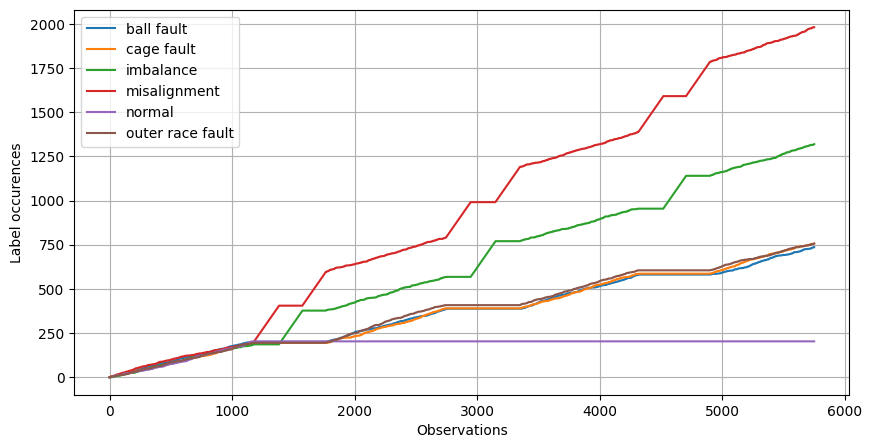
\includegraphics[width=\textwidth]{assets/design/Online-event-ordering-fault-train.png}
%        \caption{Event ordering of faults}
%        \label{fig:design:online-event-order}
%    \end{subfigure}
%    \hfill
%    \begin{subfigure}[b]{0.49\textwidth}
%        \includegraphics[width=\textwidth]{assets/design/Online-severity-levels.png}
%        \caption{Fault severity levels ordering}
%        \label{fig:design:online-count-severity-level}
%    \end{subfigure}
%    \caption{Label sequencing for progressive evaluation}
%\end{figure}

Major breaking points in the stream are after 1171 observations out of 5751, where all 203 normal conditions are consumed in the training process. Counters of other faults show that model predictions are skewed towards more represented classes of imbalance and misalignement. The uneven evolution of category counts in a stream impacts the development of accuracy in the remaining experiments. The hold-out validation accuracies of comparable batch models are 97.36\% \emph{(temporal features)} and 98.36\% \emph{(spectral features)}.
	
During gradual learning, the correct label is supplied after a fixed period passes after its prediction. This \textbf{sliding window} simulation examines accuracy every 100 iterations. Wait times before revealing the actual class associated with the sample are 1, 50, 100, or 250 steps (Fig.~\ref{fig:design:online-fault-delay-sliding}). 


%\begin{figure}[ht]
%    \centering
%    \begin{subfigure}[b]{\textwidth}
%        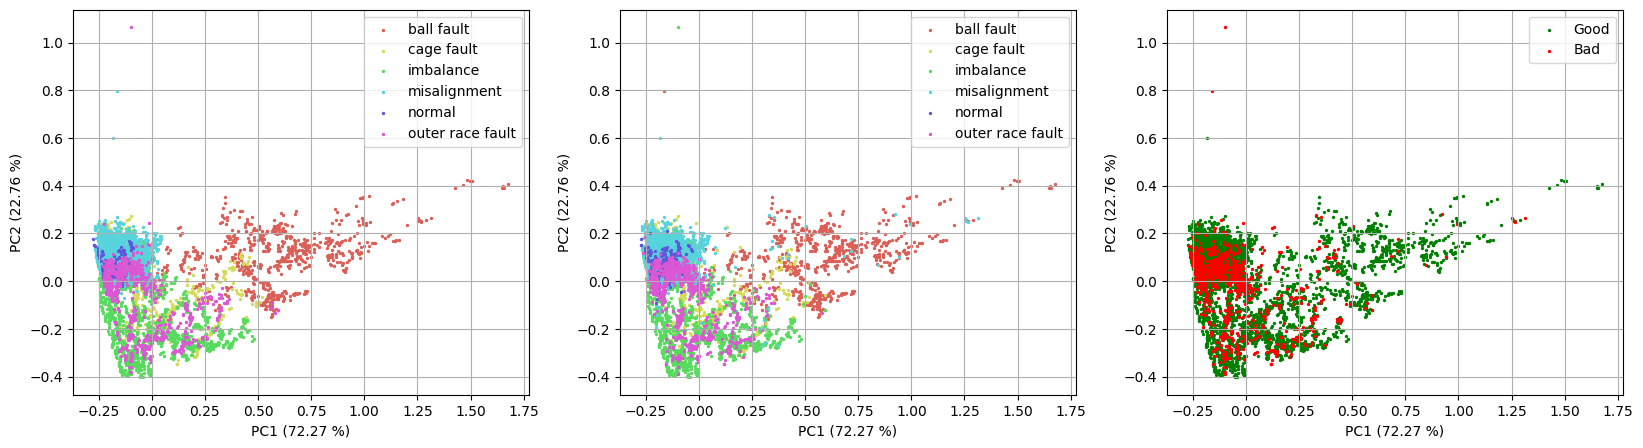
\includegraphics[width=\textwidth]{assets/design/pca-scatter-online-fault-temporal.png}
%        \caption{Principal components from temporal domain features}
%    \end{subfigure}
%    \hfill
%    \begin{subfigure}[b]{\textwidth}
%        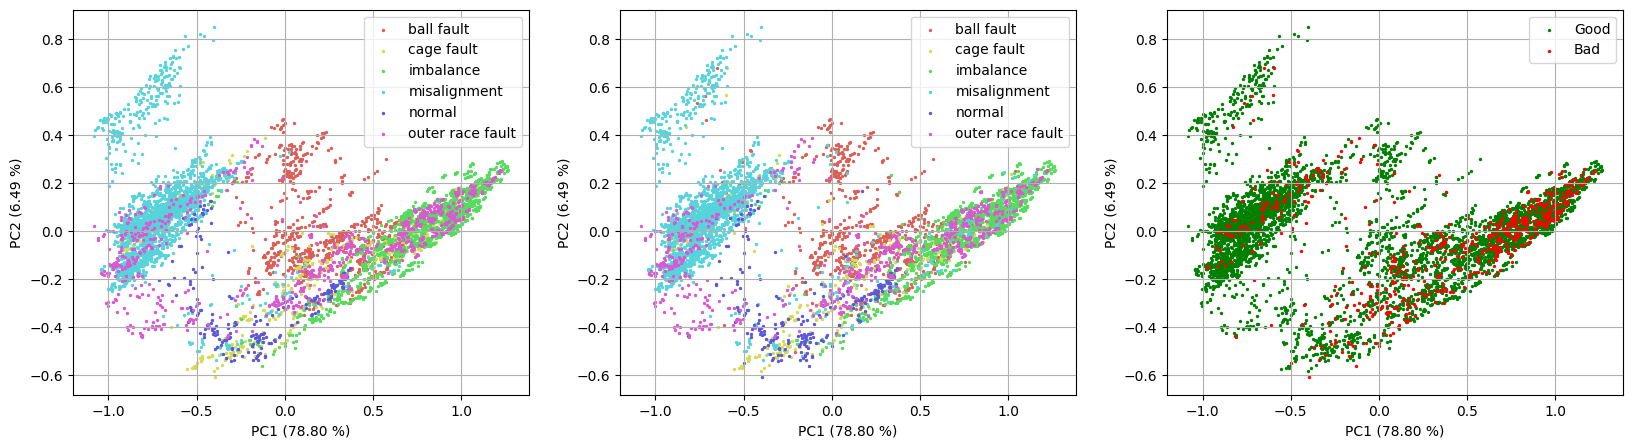
\includegraphics[width=\textwidth]{assets/design/pca-scatter-online-fault-spectral.png}
%        \caption{Principal components from spectral domain features}
%    \end{subfigure}
%    \caption{Classification labels in incremental learning \emph{(from left)}: true labels, predicted labels, mistakes in predictions.}
%    \label{fig:design:scatter-plot-online}
%\end{figure}

Accuracies after sequentially seeing all samples 96.78\% in temporal domain and 89.11\% in spectral domain when labels are shown instantly. Scatter plots in Figure~\ref{fig:design:scatter-plot-online} visualize mistakes in predictions projected onto two principal components. Labeling delay of 250 observations causes accuracy to drop to 83.94\% \emph{(temporal)} and 78.81\% \emph{(spectral)}.
	
%\begin{figure}[ht]
%    \centering
%    \begin{subfigure}[b]{0.49\textwidth}
%        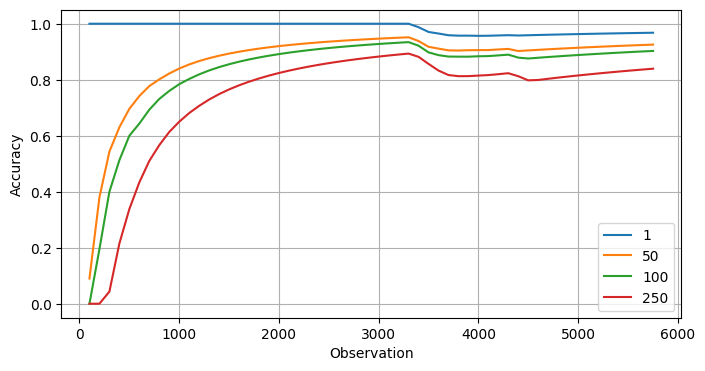
\includegraphics[width=\textwidth]{assets/design/gradual-learning-accuracy-delay-temporal-domain-fault.png}
%        \caption{Temporal domain features}
%    \end{subfigure}
%    \hfill
%    \begin{subfigure}[b]{0.49\textwidth}
%        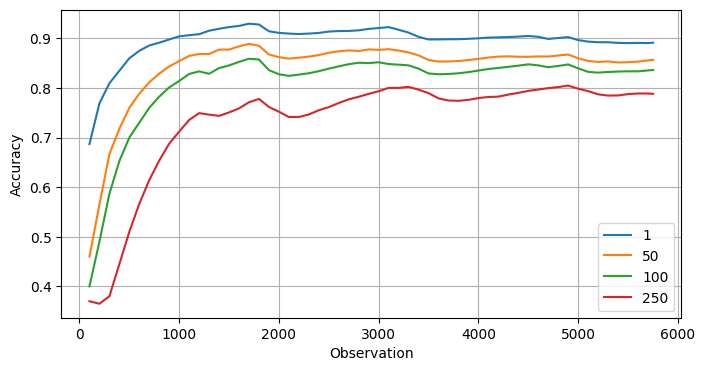
\includegraphics[width=\textwidth]{assets/design/gradual-learning-accuracy-delay-spectral-domain-fault.png}
%        \caption{Spectral domain features}
%    \end{subfigure}
%    \caption{Incremental learning on all extracted feature with delayed reveal of labels in sliding windows}
%    \label{fig:design:online-fault-delay-sliding}
%\end{figure}
	
In the final sample, the accuracies are 89.11\% \emph{(temporal)} and 90.38\% \emph{(spectral)} with immediate feedback, and 83.08\% \emph{(temporal)} and 85.01\% \emph{(spectral)} with window length of 250 samples (Fig.~\ref{fig:design:online-fault-delay-tumbling}). 

%\begin{figure}[ht]
%    \centering
%    \begin{subfigure}[b]{0.49\textwidth}
%        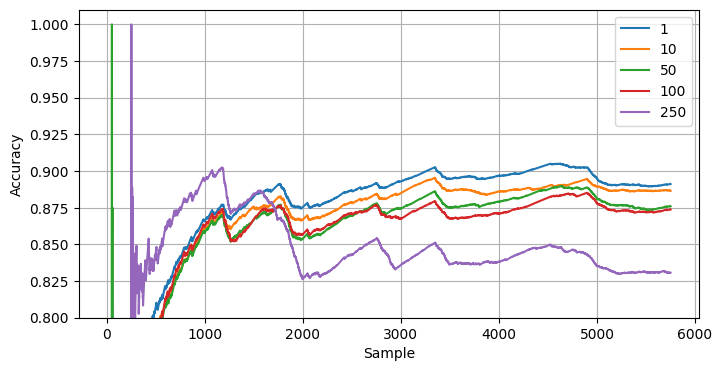
\includegraphics[width=\textwidth]{assets/design/gradual-learning-delay-temporal-domain-fault.png}
%        \caption{Temporal domain features}
%    \end{subfigure}
%    \hfill
%    \begin{subfigure}[b]{0.49\textwidth}
%        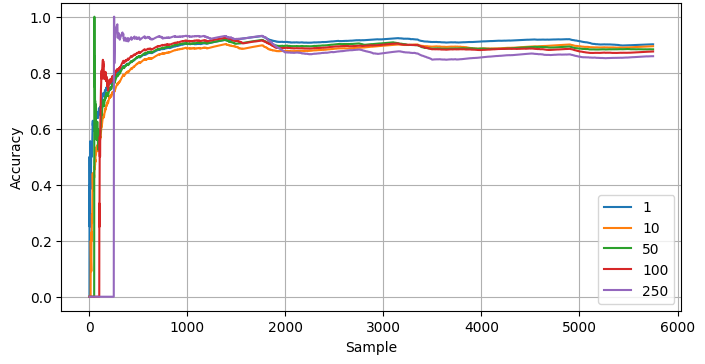
\includegraphics[width=\textwidth]{assets/design/gradual-learning-delay-spectral-domain-fault.png}
%        \caption{Spectral domain features}
%    \end{subfigure}
%    \caption{Incremental learning on all extracted feature with delayed reveal of labels at regular intervals in tumbing windows}
%    \label{fig:design:online-fault-delay-tumbling}
%\end{figure}

A \textbf{tumbling window} is more accurate according to progressive valuation because the labeling delay decreases towards the window's end. Initial 0\% accuracy is caused by a warming-up period in data collection during the span of the first few windows. The true labels are unknown. After just a handful of windows in the beginning, accuracy jumps above 60\% and stabilizes after 1000 observations.


%\begin{figure}[ht]
%    \centering
%    \begin{subfigure}[b]{0.49\textwidth}
%        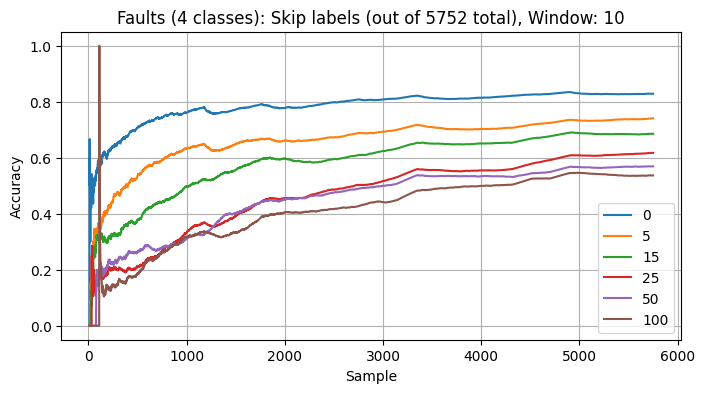
\includegraphics[width=\textwidth]{assets/design/gradual-learning-skip-temporal-domain-fault.png}
%        \caption{Temporal domain features}
%    \end{subfigure}
%    \hfill
%    \begin{subfigure}[b]{0.49\textwidth}
%        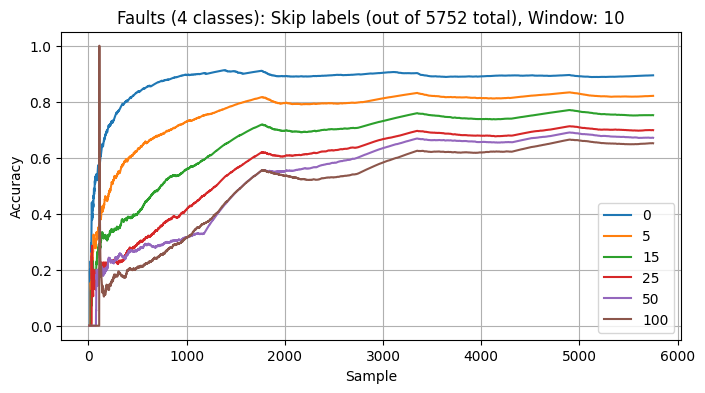
\includegraphics[width=\textwidth]{assets/design/gradual-learning-skip-spectral-domain-fault.png}
%        \caption{Spectral domain features}
%    \end{subfigure}
%    \caption{Incremental learning with missing true labels and sliding window delay of 10 observations}
%    \label{fig:design:online-label-skip}
%\end{figure}
 
Labeling just every \nth{5} sample (25\% of the total dataset) with a sliding window delay of 10 samples reduces accuracy for the model out of temporal features by 8.41\% to 80.39\%, and by 7.33\% for spectral features to accuracy of 82.01\% (Fig.~\ref{fig:design:online-label-skip}). Even if only 1\% of the dataset is annotated (every \nth{100} sample), the model out of spectral features retained an accuracy of 65.17\% that is 4.41\% better than for temporal features.  More missing labels require recording more observations before the equivalent accuracy is reached.







